\chapter{Einleitung}
\begin{figure}[h!]
	\centering
    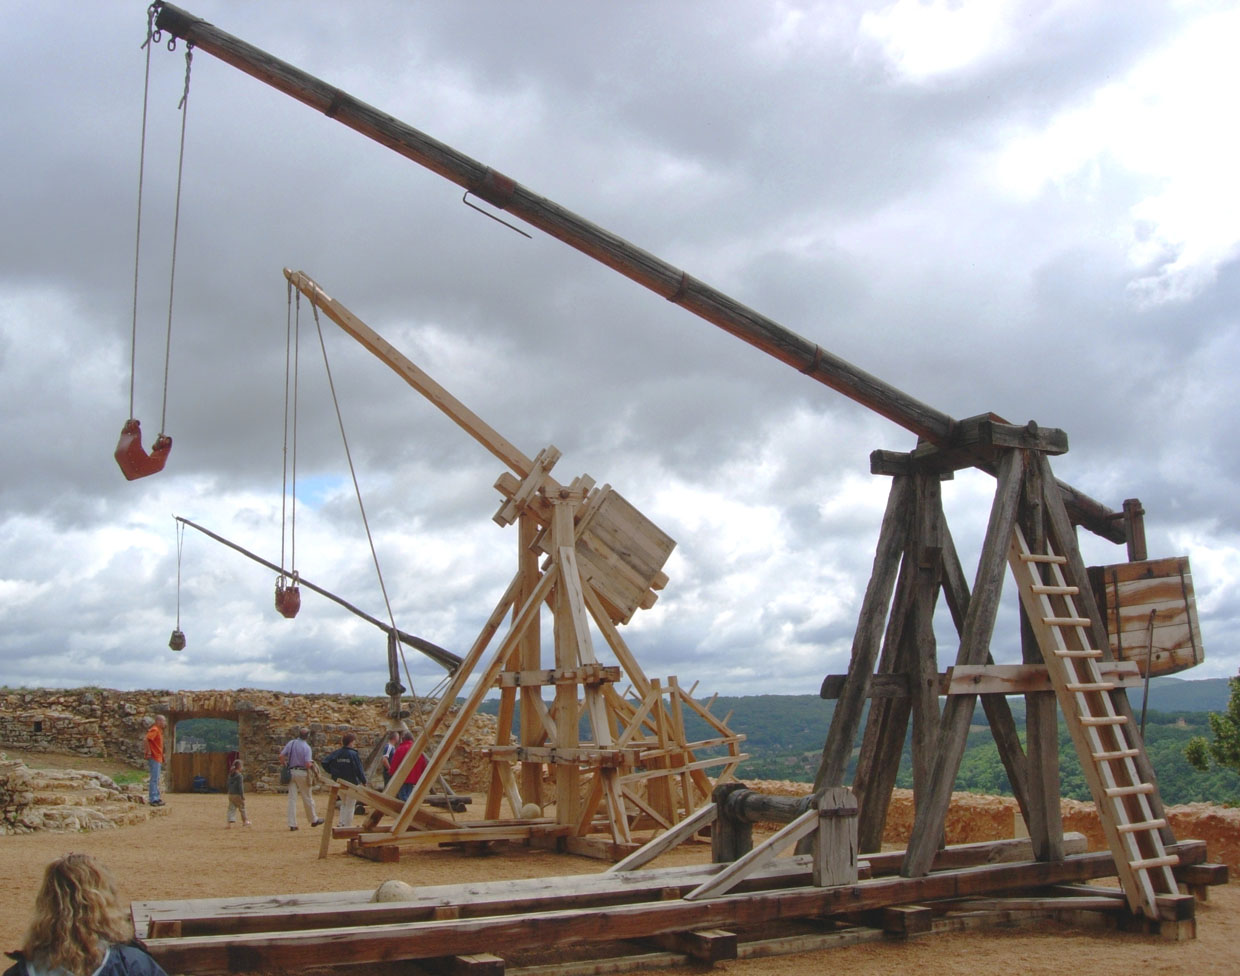
\includegraphics[width=0.5\textwidth]{bilder/Trebuchet_Castelnaud}
    \caption{Nachbau eines historischen Trebuchets. Standort: Burg Castelnaud, Südfrankreich}
    \label{bild_trebuchet}
\end{figure}

\section{Vorwort}
Das Thema einer Facharbeit in Physik sollte drei Kriterien erfüllen: Es sollte eine Erweiterung des im Unterricht durchgenommenen Stoffes darstellen, es sollte eine gewisse Komplexität aufweisen, ohne jedoch kompliziert zu sein und schließlich sollte es -nach Möglichkeit- experimentell belegbar bzw. anschaulich sein.

Welches Thema wäre daher also passender als das Trebuchet? Die Rotationsdynamik gehört nicht zum Stoff des Unterrichtes, kann sich aber mit vertretbaren Aufwand angeeignet werden, zumal einige Unterrichtsthemen schon darauf hinarbeiten (z.B. die Hebelgesetze). Bei der Herleitung der Rechnung kann (bis auf eine Ausnahme) auf einfache Schulmathematik zurückgegriffen werden, sodass sie trotz ihrer Länge nachvollziehbar bleibt.

Mit dem Trebuchet ist des Weiteren die Rotationsdynamik gut zu veranschaulichen, da man statt schlecht fassbarer Trägheitsmomente oder Winkelgeschwindigkeiten etwa die gut vorstellbare Schussweite ausrechnen kann. Mit einem interessanten Experiment kann ferner nicht nur die Richtigkeit der Berechnungen belegt, sondern auch das Experiment optimiert werden.

Neben meinem persönlichen Interesse ist das Trebuchet also ein spannendes und angemessenes Thema, das eines genaueren Blicks wert ist.

Diese Facharbeit beschäftigt sich im Besonderen mit der Frage, wie weit ein Trebuchet schießen kann. Dies ist, neben der Schusshöhe, die interessanteste und anschaulichste Problemstellung. Dabei wird die für die Fragestellung relevante Mechanik starrer Körper definiert und angewandt, um diese Frage angemessen zu beantworten.

\section{Das Trebuchet}
Das Trebuchet, im deutschen Raum auch \emph{Bilde} oder \emph{Tribock} genannt, ist eine Belagerungswaffe aus dem Hochmittelalter. Es wurde vermutlich um 1097 erfunden und -trotz der Einführung des Schießpulvers im 13. Jahrhundert- bis ins 15. Jahrhundert hinein benutzt.

Die Grundkonstruktion des Trebuchets besteht aus einem Hebel mit einem kurzen und einem langen Arm. Am Ende des kurzen Arms ist ein sogenanntes Gegengewicht befestigt, das den Antrieb der Waffe darstellt. Am Ende des langen Arms befindet sich ein Geschoss, welches beim Hinunterfallen des Gegengewichtes geschleudert wird. Weil das Trebuchet also keine Federn, Seile oder ähnliches als Antrieb benutzt, konnte es in fast beliebiger Größe und aus gut verfügbaren Materialien gebaut werden, sodass es eine der verheerendsten und ausgereiftesten Waffen des Mittelalters wurde.